\documentclass[../../index]{subfiles}

\begin{document}
\chapter{コンピュータとマルチメディア}
この章では,コンピュータで文字・画像を扱うにあたっての基礎知識を解説する.
また,他者が製作した文書・画像を利用するときに重要となる,ライセンスについても説明する.

\section{文字コード}
コンピュータにおいて,テキストを記録するには,テキストを数値の列に変換しなければならない.
この変換方式のことを\termdef{文字コード}\index{もじこーど@文字コード}という.
文字コードは複数あり,それぞれ利用できる文字や変換方式などが異なる.

\begin{floatingfigure}{\smallfiguresize}
  \centering
  \tcbincludegraphics[myframe,width=\smallfiguresize]{notepad.png}
  \caption{Windows 10のメモ帳}
\end{floatingfigure}

たとえば,最新のWindows 10にあるメモ帳でテキストを保存すると,UTF-8\index{utf8@UTF-8}という方式で
文字列が数値の列に変換される.この他にも,ソフトウェアに応じてASCII\index{ascii@ASCII},Shift\_JIS\index{shiftjis@Shift\_JIS}など,
さまざまな文字コードが利用されている.

現在では\termdef{Unicode}\index{unicode@Unicode}という文字コードの規格が主流になりつつある.
先述のUTF-8も,このUnicodeにおいて定義されている.
この節では文字コードの代表例として,Unicodeについて解説する.
なお,以下に示す用語は文字コードによっては異なる名前で呼ばれることもあるし,対応する概念が無いこともある.

文字コードが扱える文字の全体集合を\termdef{文字集合}\index{もじしゅうごう@文字集合}という.
文字集合の各要素には固有の非負整数が割り当てられており,
その対応関係をUnicodeでは\termdef{符号化文字集合}\index{ふごうかもじしゅうごう@符号化文字集合}と呼ぶ
\footnote{対応関係なのに集合? と思うのももっともだが,公式資料には確かに「a mapping from an abstract character repertoire to a set of nonnegative integers」\cite{Whistler2008}とある.}.

符号化文字集合(の像)は,集合\(S=\Set{0_{(16)},\dots,\literal{10FFFF}_{(16)}}\)の真部分集合である.
\(S\)を\termdef{符号空間}\index{ふごうくうかん@符号空間}といい,\(S\)の要素を\termdef{符号位置}\index{ふごういち@符号位置}という.
符号位置は,十六進数の先頭に「U+」を付けて「U+304B」のようにして表される.

符号化文字集合は,数値を並べたときに区切れ目がただ1通りに定まるかどうかを考慮していない.
そこで,あとから区切れ目が分かるように,符号化文字集合(の像)に属する数値を整数の組\footnote{正確には1バイトの組である.}(\termdef{符号単位}\index{ふごうたんい@符号単位})へと変換する規則が必要になる.
この規則を\termdef{文字符号化形式}\index{もじふごうかけいしき@文字符号化形式}といい,UTF-8,UTF-16\index{utf16@UTF-16},UTF-32\index{utf32@UTF-32}の3つが定義されている.

\begin{figure}[htb]
  \centering
  \begin{tikzcd}
    \text{か} \arrow[r,"\text{符号位置に変換}"]
    &[6\zw] \text{U+304B} \arrow[r,"\text{符号単位に変換}"]
    &[6\zw] \text{\texttt{E3 81 8B}}
  \end{tikzcd}
  \caption{文字の符号単位への変換}
  \label{figure:character_to_byte_sequence}
\end{figure}

\cref{table:unicode_code_point}にUnicodeの符号化文字集合を一部抜粋して示す.

\begin{table}[htb]
  \centering
  \caption{符号化文字集合の一部}
  \label{table:unicode_code_point}
  \begin{tabular}{c|ccccccc} \hline
    U+   &      0     &      1      &      2     &      3     &      4     &      5     &      6     \\ \hline
    0020 & \UTF{0020} & \UTF{0021}  & \UTF{0022} & \UTF{0023} & \UTF{0024} & \UTF{0025} & \UTF{0026} \\
    0030 & \UTF{0030} & \UTF{0031}  & \UTF{0032} & \UTF{0033} & \UTF{0034} & \UTF{0035} & \UTF{0036} \\
    0040 & \UTF{0040} & \UTF{0041}  & \UTF{0042} & \UTF{0043} & \UTF{0044} & \UTF{0045} & \UTF{0046} \\ \hline
  \end{tabular}
\end{table}

例として「M系列」という文字列について考えよう.
「M系列」の各文字をUnicodeの符号位置に置き換えると次のようになる.
\begin{codeblock}
U+004D U+7CFB U+5217
\end{codeblock}

そして,これらをUTF-8で符号単位の列に変換すると次のようになる
\footnote{UTF-16とUTF-32では符号単位の列をバイト列に変換する方法(\termdef{文字符号化スキーム}\index{もじふごうかすきーむ@文字符号化スキーム})も問題になる.UTF-8では,符号単位を並べたものをそのままバイト列とする.}.
「\inlinecode{4D}」がU+004D,「\inlinecode{E7 B3 BB}」がU+7CFB,「\inlinecode{E5 88 97}」がU+5217にそれぞれ対応する.
\begin{codeblock}
4D E7 B3 BB E5 88 97
\end{codeblock}

\section{ラスタ形式とベクタ形式}
コンピュータで画像を記録する方法は,\termdef{ラスタ形式}\index{らすたけいしき@ラスタ形式}と\termdef{ベクタ形式}\index{べくたけいしき@ベクタ形式}の2つに大別される.
ラスタ形式は,画像を単色の要素(\termdef{画素}\index{がそ@画素})を集めたものとして記録する方法である.
これに対し,ベクタ形式は画像を図形の集まりとして記録する方法である.

例を挙げると,\termdef{JPEG}\index{jpeg@JPEG},\termdef{PNG}\index{png@PNG}はラスタ形式である.
また,ベクタ形式である\termdef{SVG}\index{svg@SVG}は,Webページのデザインにしばしば利用されている.

ベクタ形式に比べ,ラスタ形式は拡大・縮小の影響を受けやすい.ラスタ形式の画像を拡大したときの様子を\cref{figure:raster_scaling}に示す
(ただし,ラスタ形式の画像を拡大・縮小した結果は利用したソフトウェアに依存する.詳しくは\cref{subsection:raster_scaling}を参照のこと).

\begin{figure}[htb]
  \begin{subfigure}{0.5\linewidth}
    \centering
    \tcbincludegraphics[myframe,width=\smallfiguresize]{graph.png}
    \caption{画像全体}
  \end{subfigure}%
  \begin{subfigure}{0.5\linewidth}
    \centering
    \tcbincludegraphics[myframe,width=\smallfiguresize]{raster_scaling.png}
    \caption{中央付近を拡大}
  \end{subfigure}
  \caption{ラスタ形式の画像を拡大したときの様子}
  \label{figure:raster_scaling}
\end{figure}

これに対し,ベクタ形式の画像は拡大しても\cref{figure:raster_scaling}のようにならない.
これは,ベクタ形式では拡大・縮小に応じて図形を描画しなおせるからである.
ベクタ形式の画像を拡大したときの様子を\cref{figure:vector_scaling}に示す.

\begin{figure}[htb]
  \begin{subfigure}{0.5\linewidth}
    \centering
    \tcbincludegraphics[myframe,width=\smallfiguresize]{graph.png}
    \caption{画像全体}
  \end{subfigure}%
  \begin{subfigure}{0.5\linewidth}
    \centering
    \tcbincludegraphics[myframe,width=\smallfiguresize]{vector_scaling.png}
    \caption{中央付近を拡大}
  \end{subfigure}
  \caption{ベクタ形式の画像を拡大したときの様子}
  \label{figure:vector_scaling}
\end{figure}

\section{可逆圧縮と非可逆圧縮}
この節では,ラスタ形式の画像について扱う.
多くの場合,ラスタ形式の画像ファイルは,データサイズを削減するために圧縮されている.
圧縮した後のデータから元のデータを復元できる圧縮方式を\termdef{可逆圧縮}\index{かぎゃくあっしゅく@可逆圧縮},
復元できない圧縮方式を\termdef{非可逆圧縮}\index{ひかぎゃくあっしゅく@非可逆圧縮}という.

たとえば,PNGは可逆圧縮,JPEGは非可逆圧縮である\footnote{JPEGの規格は可逆圧縮にも対応している.しかし,多くの場合JPEGは非可逆圧縮に利用されるので,本書ではJPEGは非可逆圧縮であると見なす.}.
非可逆圧縮のほうがデータサイズが小さくなる傾向にあるが,画像の性質にもよるので一概には言えない.
大雑把に言うと,PNGは線画,JPEGは写真に強い傾向にある.

非可逆圧縮を利用するときは,圧縮するたびに画像が劣化することに注意しなければならない.
また,データサイズを削減するために品質をあまりに低く設定すると,
画像が非常に粗くなることがある.\cref{figure:image_compression}に,JPEGの
品質(0以上100以下の整数を設定できる)を10に設定して圧縮したときの様子を示す.

\begin{figure}[htbp]
  \centering
  \begin{subfigure}{0.5\linewidth}
    \centering
    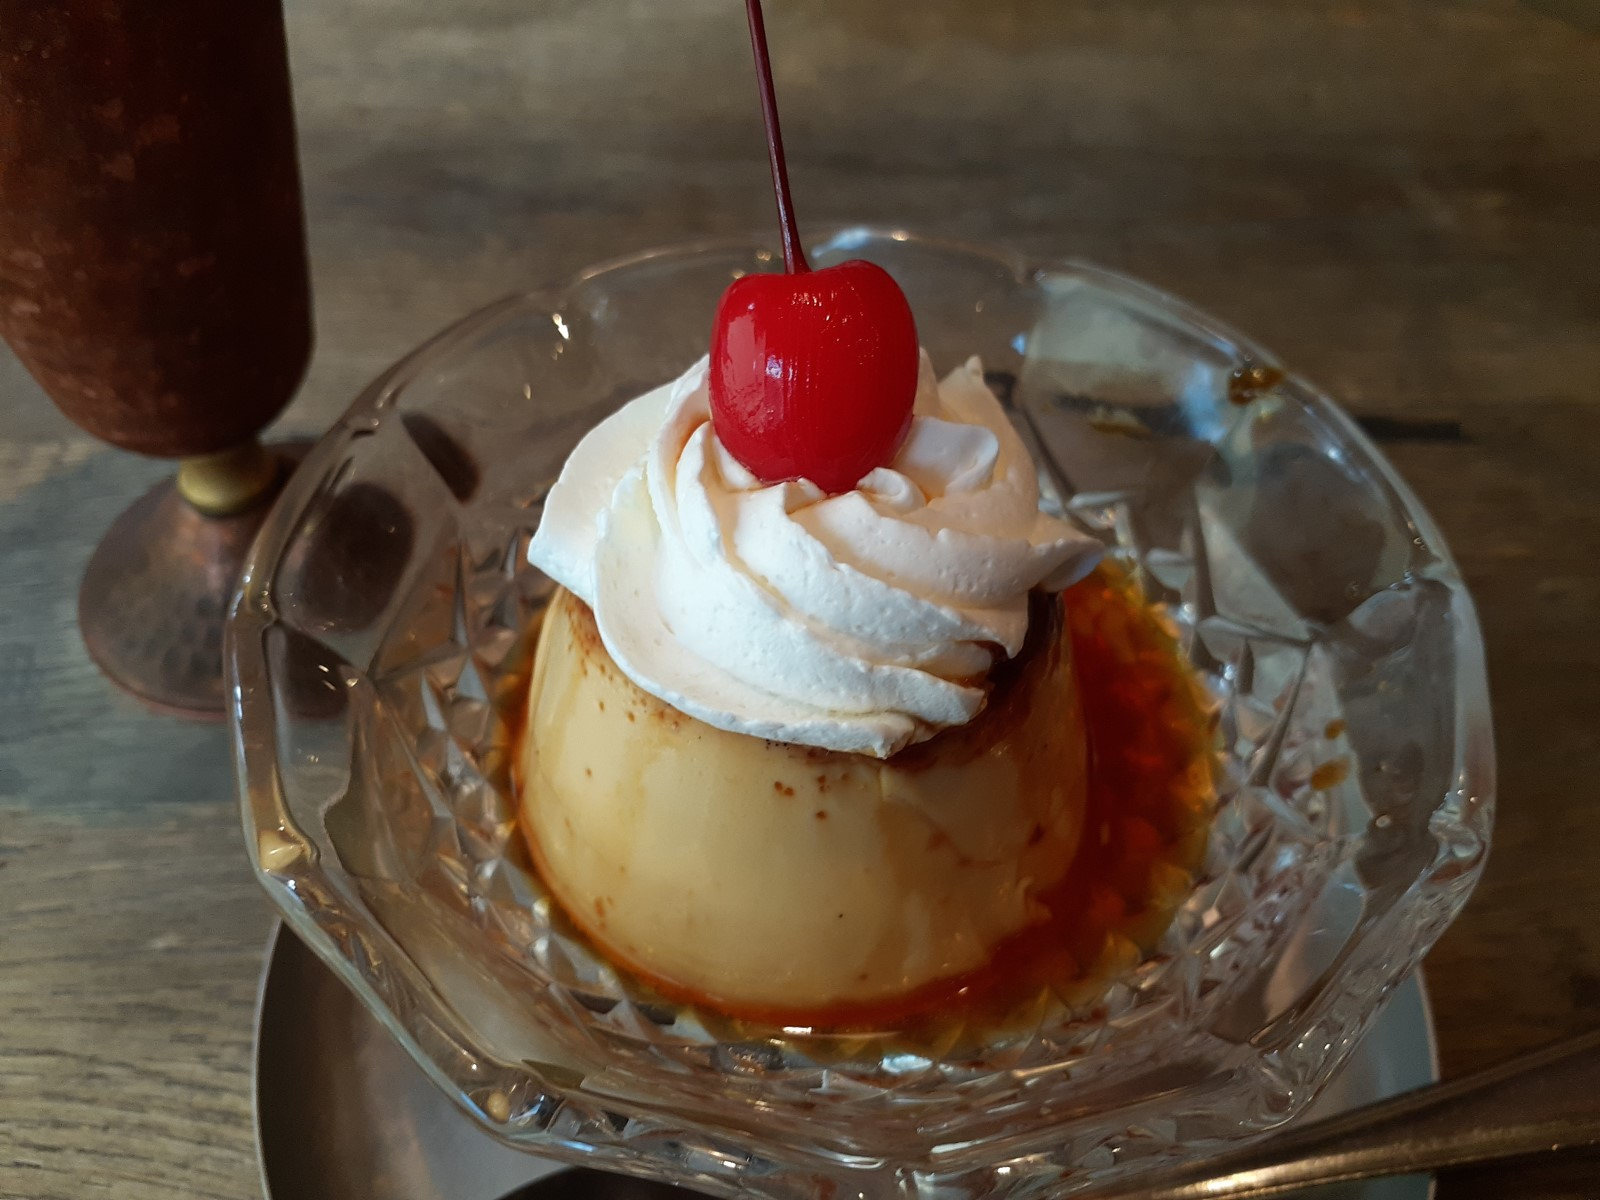
\includegraphics[width=\smallfiguresize]{pudding.jpeg}
    \caption{元画像}
  \end{subfigure}%
  \begin{subfigure}{0.5\linewidth}
    \centering
    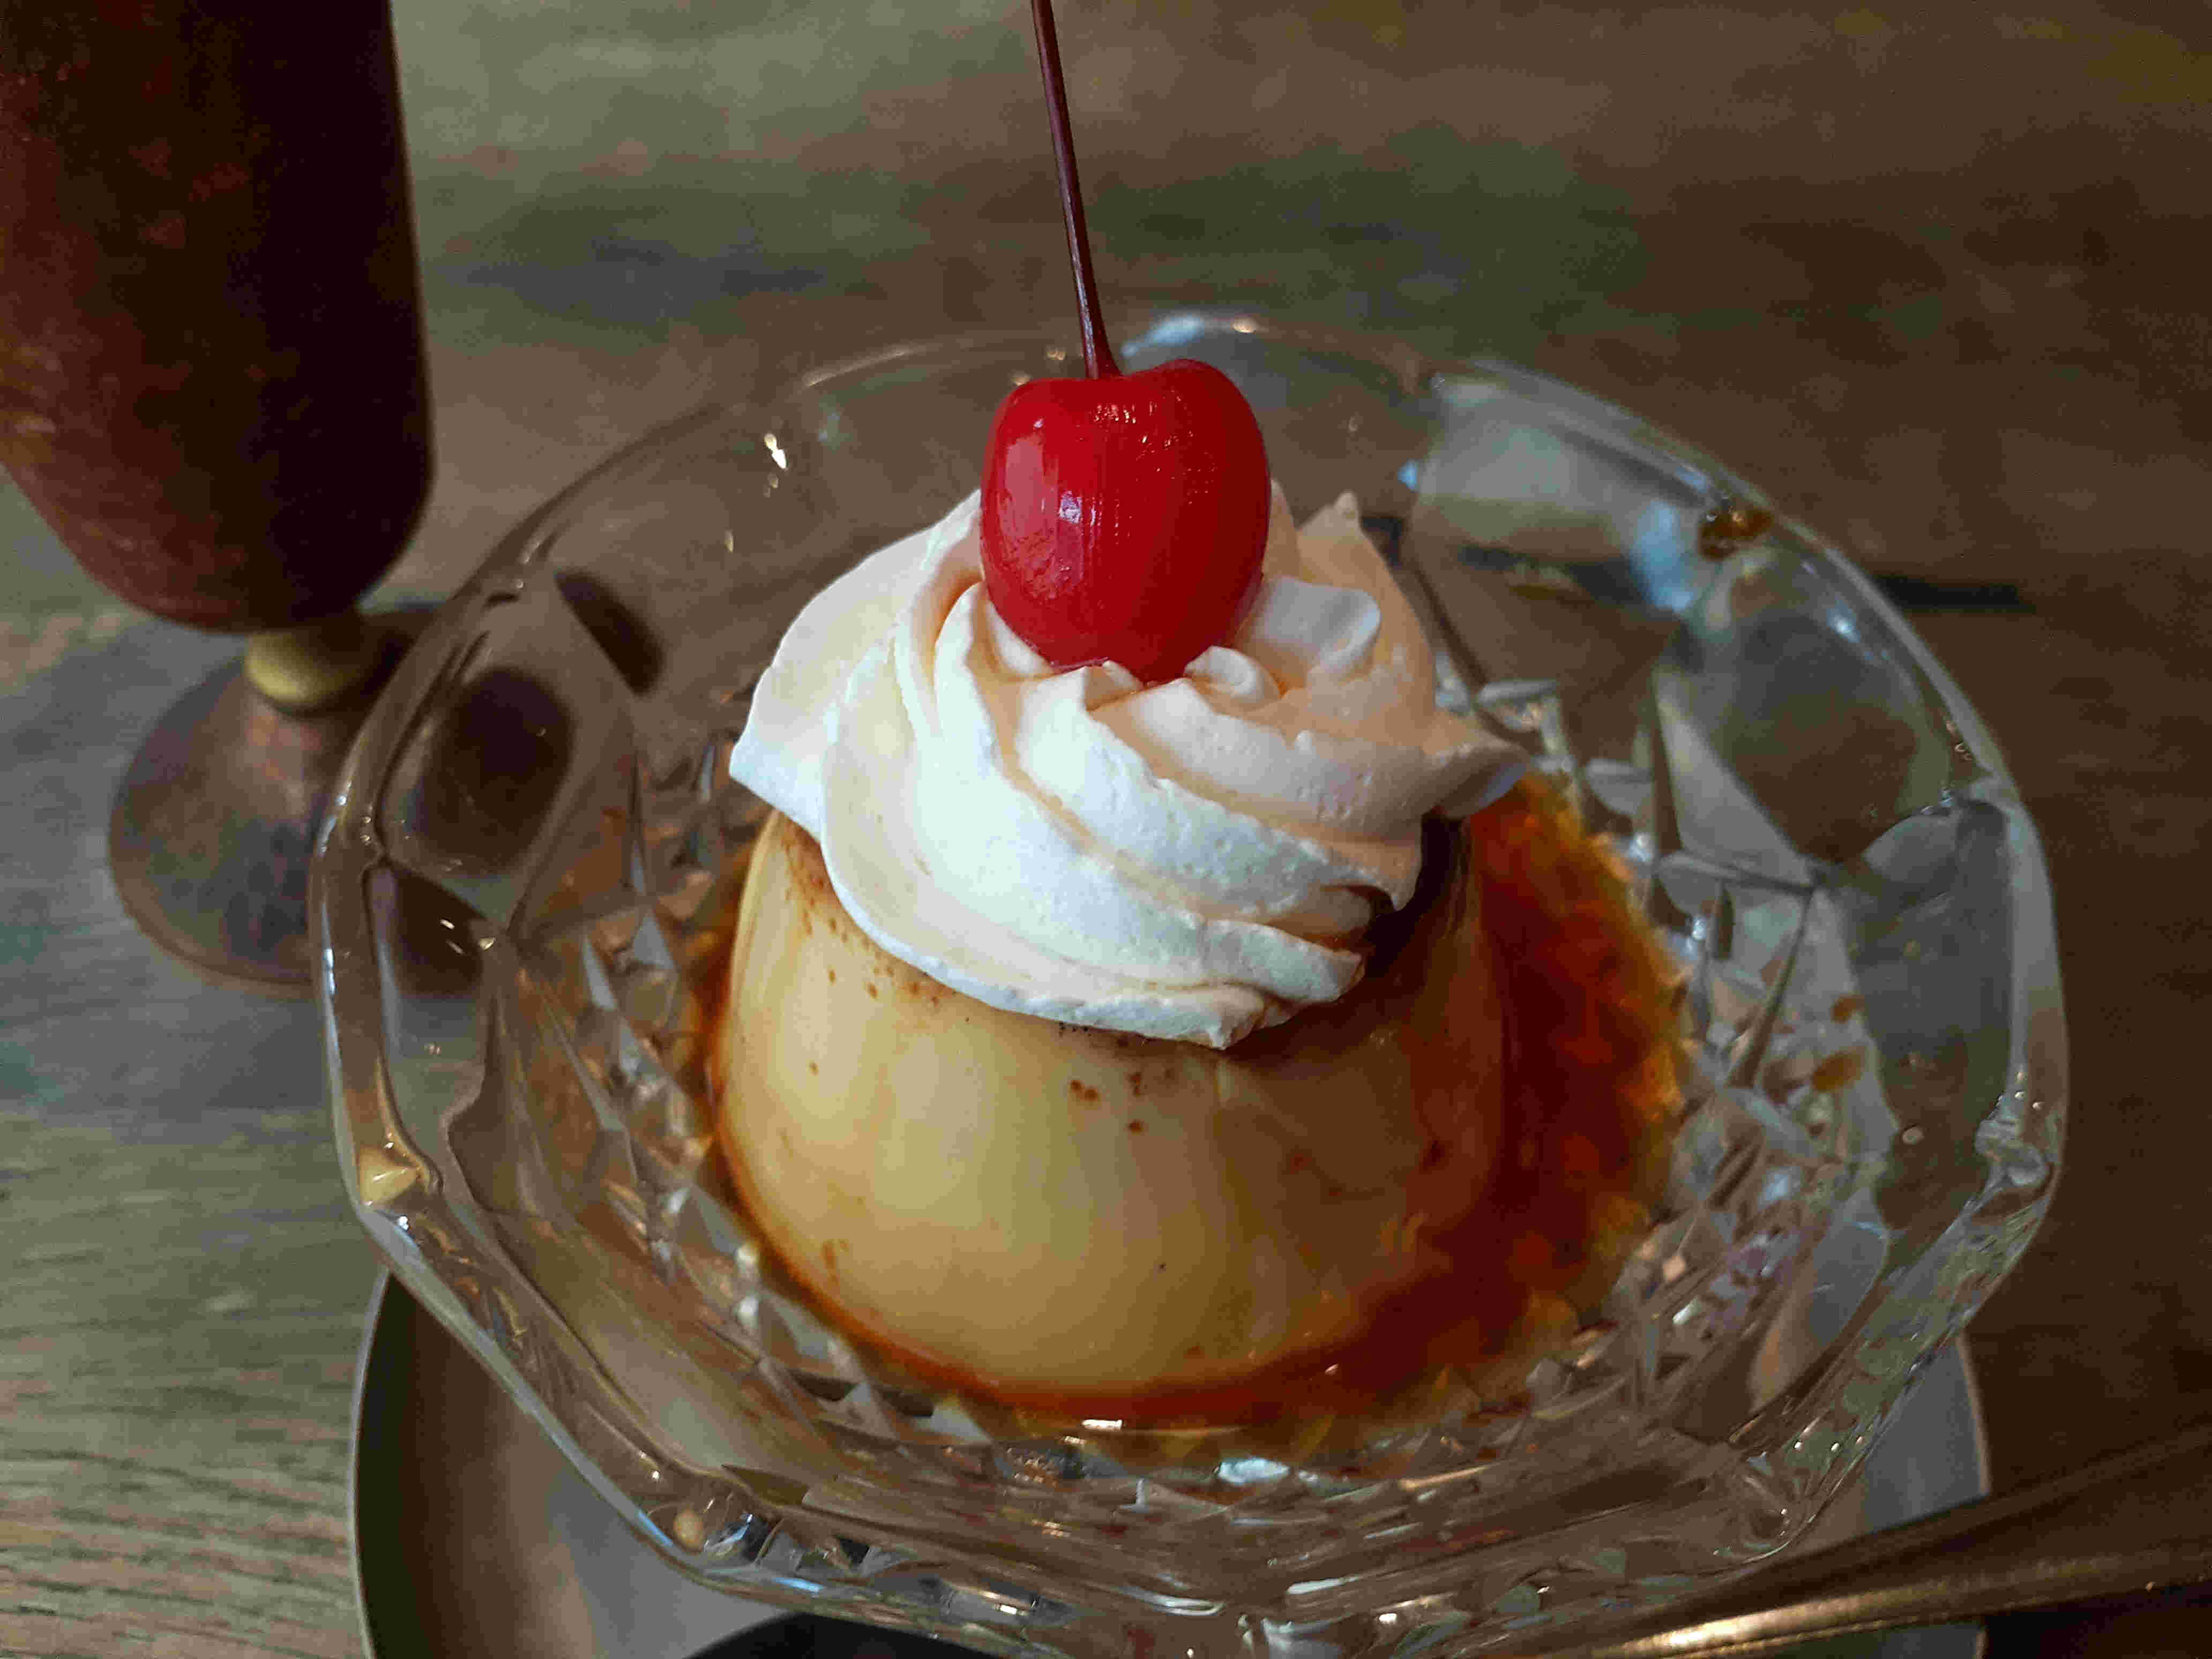
\includegraphics[width=\smallfiguresize]{worse.jpeg}
    \caption{圧縮した画像}
  \end{subfigure}
  \caption{画像の過剰な圧縮に伴う劣化}
  \label{figure:image_compression}
\end{figure}

\section{ライセンス}
通常,製作者は自身の製作物に関して知的財産権を持つ.
したがって,他者の製作物を利用するとき,普通は製作者に対して許可をとる必要がある\footnote{適正な範囲での引用など,例外はある.\cite{bunka}にこうした例外が列記されている.}.
しかし,製作物の\termdef{ライセンス}\index{らいせんす@ライセンス}が明記されていれば,
利用者はライセンスと法律の範囲内で自由に製作物を利用できる(もちろん,良識のない利用は慎むべきである).

たとえば,本書は\href{https://creativecommons.org/licenses/by-nc-nd/4.0/deed.ja}{CC BY-NC-ND 4.0}というライセンスの下で配布されている.
したがって,読者は自由に本書を再配布できる.しかし,本書を改変した場合は再配布できないなど,いくつかの制約が課される.

\section{補遺}
\subsection{文字化けの仕組み}
\begin{floatingfigure}{\smallfiguresize}
  \centering
  \tcbincludegraphics[myframe,width=\smallfiguresize]{mojibake.png}
  \caption{文字化けしたテキスト}
  \label{figure:mojibake}
\end{floatingfigure}

多くの場合,文字化けはテキストの文字コードをソフトウェアが誤判定したときに発生する.
たとえば,\cref{figure:mojibake}ではUTF-8で作成したテキストをShift\_JISで開いてしまっている.

文字化けを直すには,適切な文字コードを指定してテキストを開きなおせばよい.
Visual Studio Code\index{visualstudiocode@Visual Studio Code}\footnote{\url{https://code.visualstudio.com}}などのテキストエディタは,ユーザが文字コードを選択しなおす機能を備えている.

また,テキストをUTF-8で符号化したにもかかわらず,テキストエディタが文字コードをASCIIと判定する場合がある.
これは,UTF-8とASCIIの仕様には共通する部分があるので,
たまたまテキスト中の文字がすべてASCIIの文字集合にも属していた場合,文字コードをどちらとも解釈できることがあるからである.

\subsection{ラスタ形式と拡大・縮小}
\label{subsection:raster_scaling}
ラスタ形式の画像に対する拡大・縮小は,元の画像から新たな画像を作成する操作と言える.
そのため,拡大・縮小の手法は複数存在する.
\termdef{ニアレストネイバー法}\index{にあれすとねいばーほう@ニアレストネイバー法},
\termdef{バイリニア法}\index{ばいりにあほう@バイリニア法},
\termdef{バイキュービック法}\index{ばいきゅーびっくほう@バイキュービック法}
は,よく知られた拡大・縮小の手法である.各手法で画像を拡大したときの様子を\cref{figure:image_scaling_comparison}に示す.
ただし,\cref{figure:image_scaling_comparison}の画像編集はすべてGIMP\footnote{\url{https://www.gimp.org}}で行った.
また,各手法の特徴が分かりやすくなるように,(b)から(d)は(a)の画像を幅が100pxになるまでニアレストネイバー法で縮小してから,幅が1600pxになるまで拡大した.

\begin{figure}[htbp]
  \centering
  \begin{subfigure}{0.5\linewidth}
    \centering
    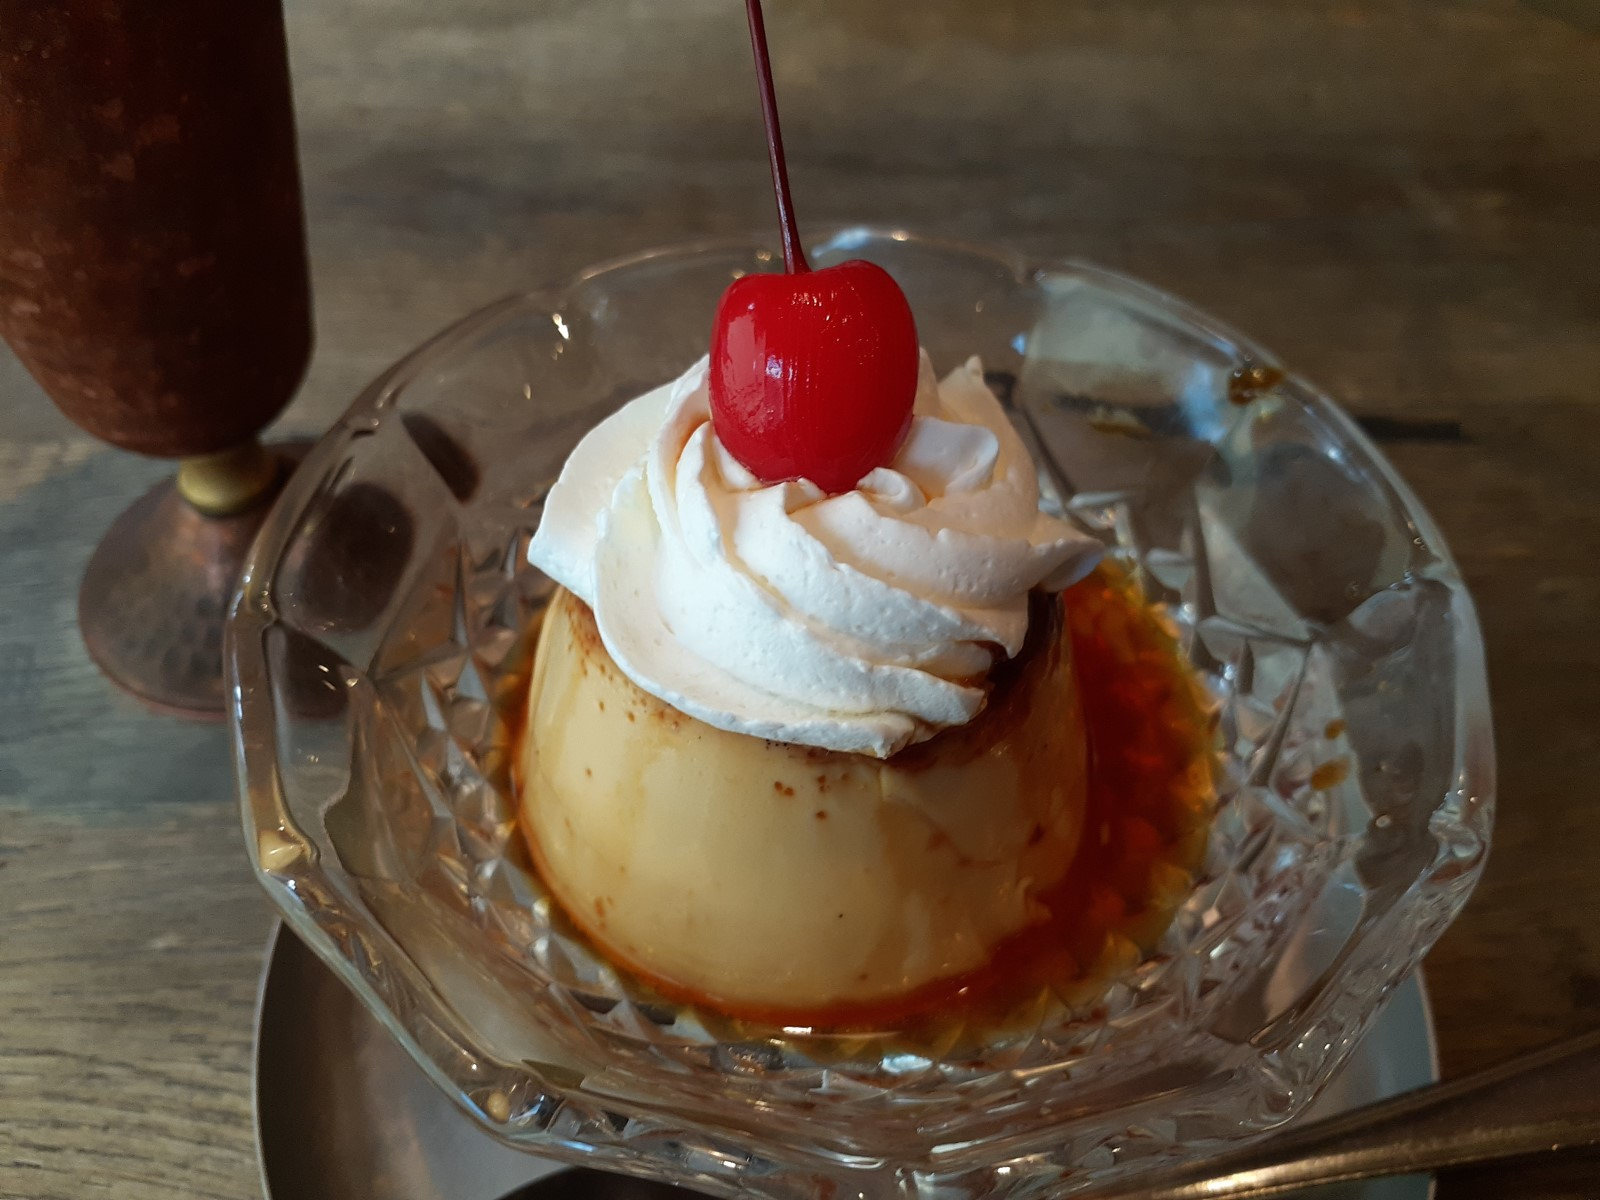
\includegraphics[width=\smallfiguresize]{pudding.jpeg}
    \caption{元画像}
  \end{subfigure}%
  \begin{subfigure}{0.5\linewidth}
    \centering
    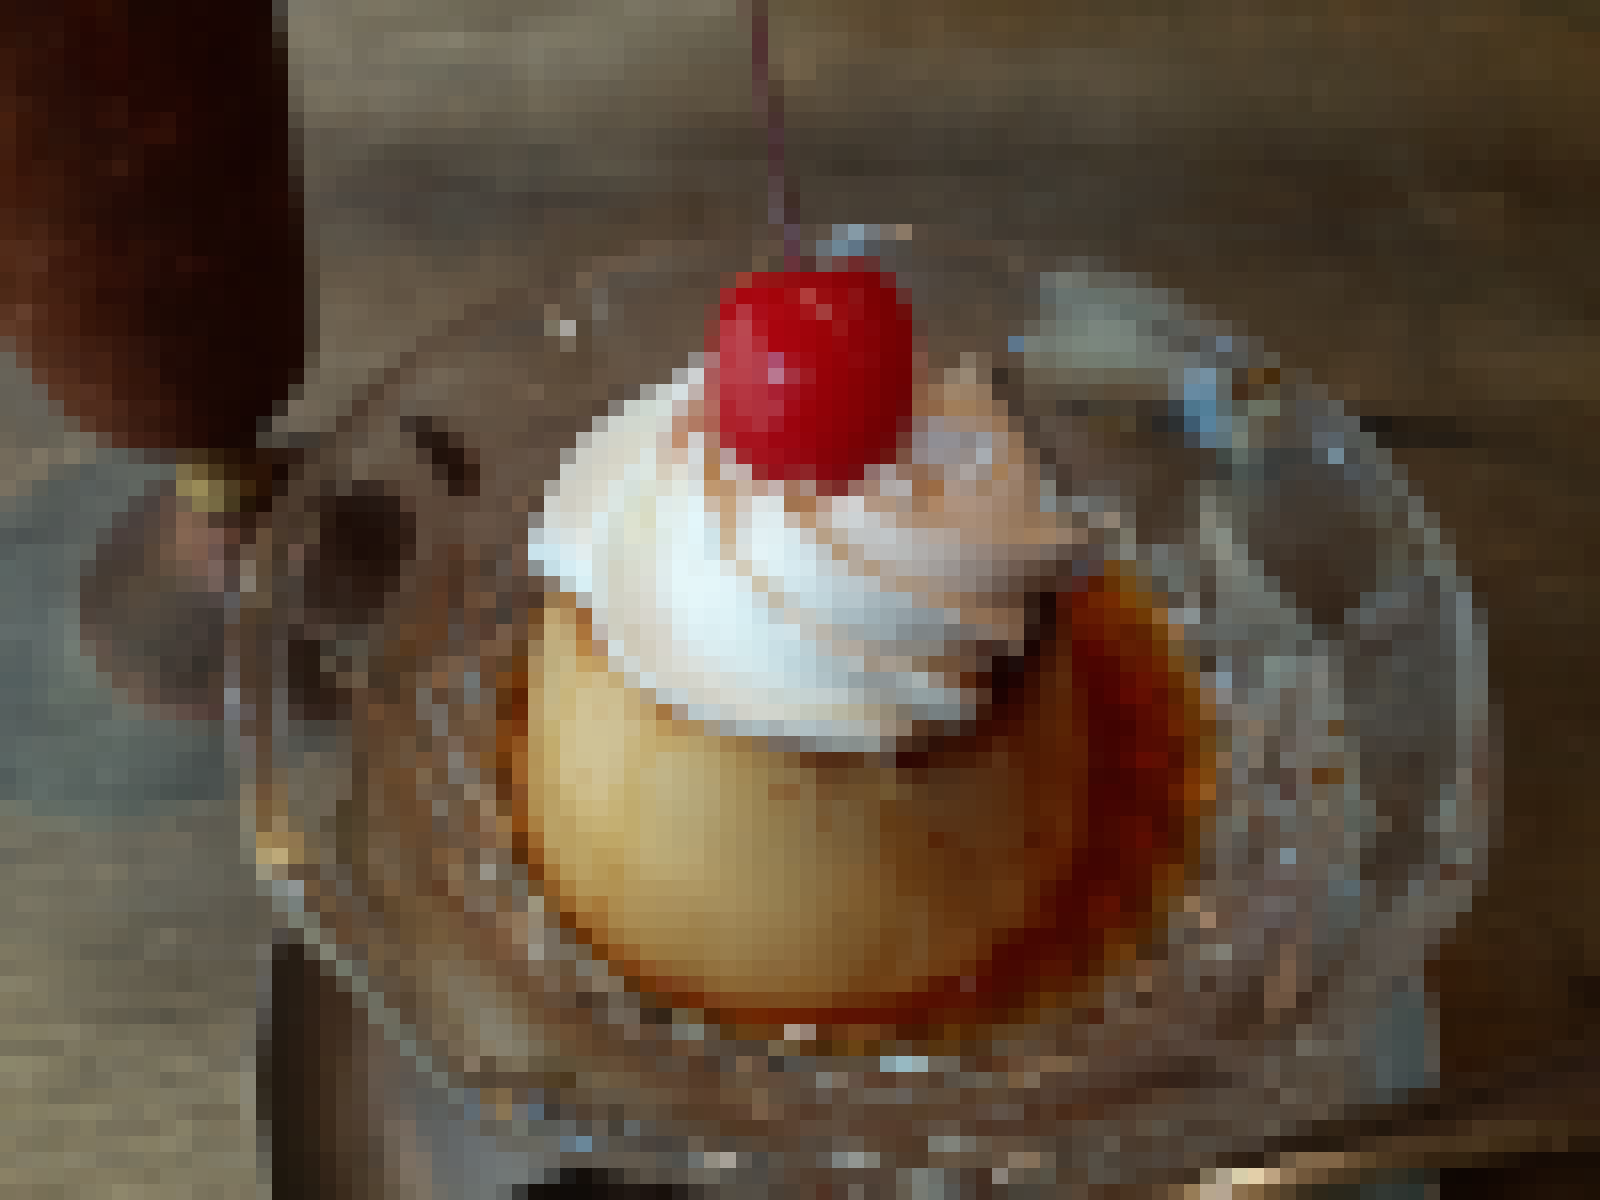
\includegraphics[width=\smallfiguresize]{nearest.png}
    \caption{ニアレストネイバー法}
  \end{subfigure}
  \hfill\vspace{\baselineskip}
  \begin{subfigure}{0.5\linewidth}
    \centering
    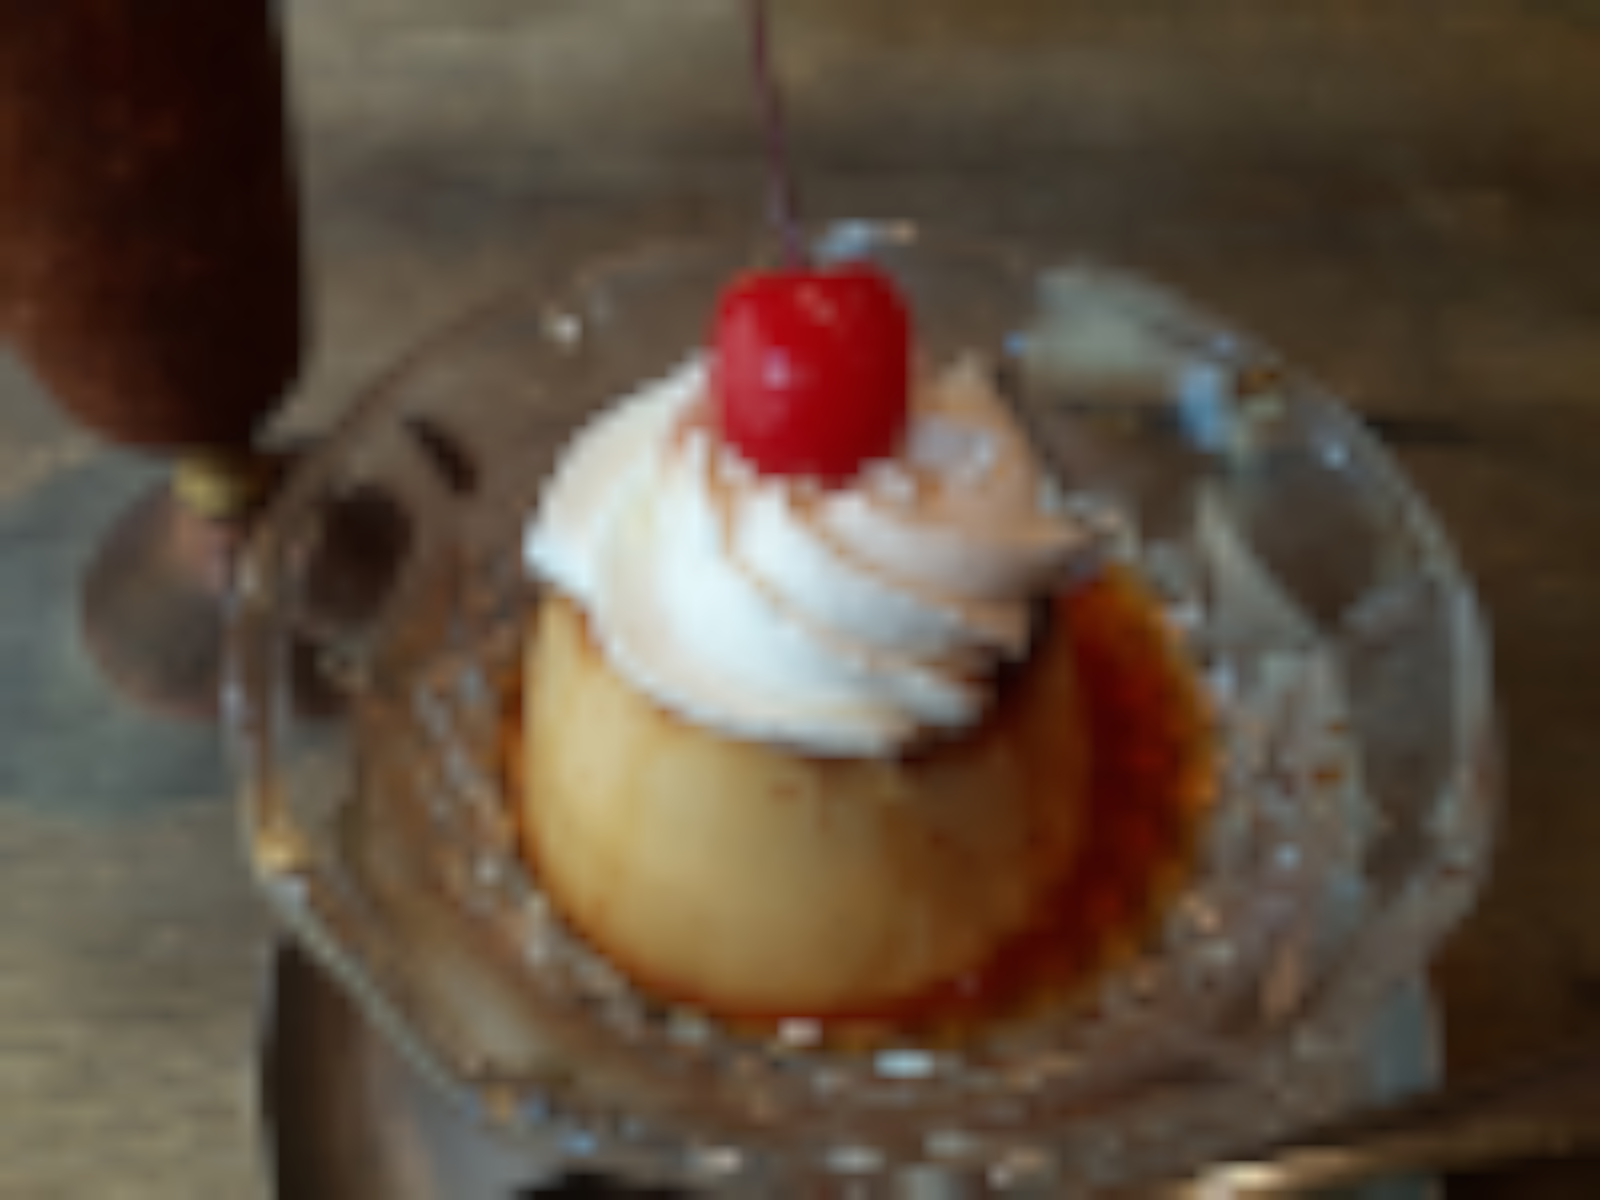
\includegraphics[width=\smallfiguresize]{linear.jpeg}
    \caption{バイリニア法}
  \end{subfigure}%
  \begin{subfigure}{0.5\linewidth}
    \centering
    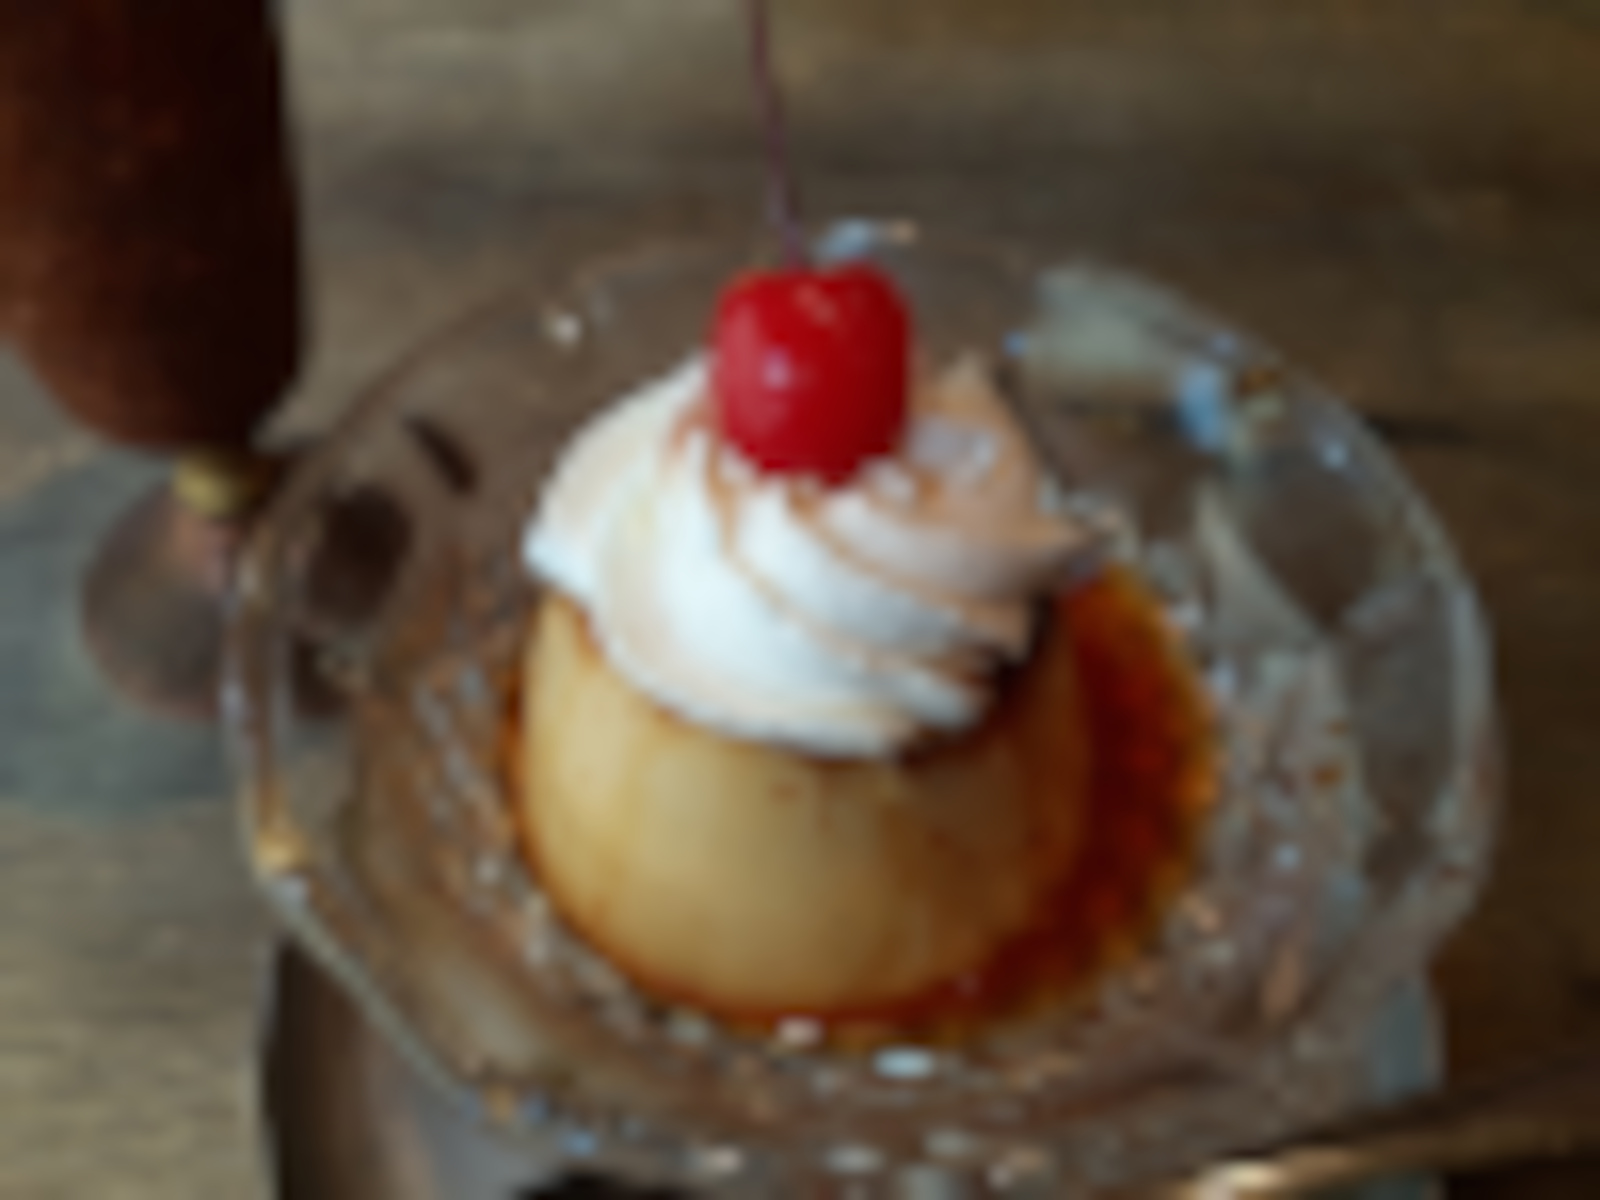
\includegraphics[width=\smallfiguresize]{bicubic.jpeg}
    \caption{バイキュービック法}
  \end{subfigure}
  \caption{画像の拡大手法の比較}
  \label{figure:image_scaling_comparison}
\end{figure}

\cref{figure:image_scaling_comparison}において生クリームの境界線に注目すると,
拡大結果がバイキュービック法,バイリニア法,ニアレストネイバー法の順になめらかであることが分かる.

\cref{figure:image_scaling_comparison}で挙げた以外にも,
画像が粗くなるのを回避するために機械学習を応用した手法が提案されていたりと\cite{dong2014},
様々な手法が研究されている.

\end{document}
